\chapter{Object-Oriented Programming}

\section{What is OOP}

\begin{itemize}
    \item OOP is a programming paradigm that revolves around objects.
    \item Objects represent instances of classes, encapsulating data \textbf{and behavior}.
    \item Key principles include encapsulation, inheritance, and polymorphism.
\end{itemize}

\begin{definitionblock}
    
    \textbf{OOP in C++}
    
    C++ is not (only) an OOP language. It is a \textbf{multi-paradigm programming language} that supports procedural, object-oriented, and generic programming. 
    
    C++ allows developers to combine these paradigms effectively for various programming tasks.
\end{definitionblock}

\section{Key Principles of OOP}

Object-Oriented Programming (OOP) is a programming paradigm that emphasizes the use of objects to represent real-world entities and concepts. It is based on several key principles:

\begin{itemize}
    \item \textbf{Encapsulation}: Encapsulation bundles data (attributes) and the functions (methods) that operate on the data into a single unit called an \textit{object}. This promotes data hiding and reduces the complexity of the code.
    \item \textbf{Inheritance}: Inheritance allows you to create new classes (derived or child classes) based on existing classes (base or parent classes). It enables code reuse and the creation of class hierarchies.
    \item \textbf{Polymorphism}: Polymorphism allows objects of different classes to be treated as objects of a common base class. It promotes code flexibility and the ability to work with objects at a higher level of abstraction.
\end{itemize}

\section{RAII Idiom (Resource Acquisition Is Initialization)}

\textbf{Holding a resource is a class invariant, tightly bound to the object's lifetime}

\begin{enumerate}
    \item Encapsulate a resource within a class (constructor).
    \item Utilize the resource through a local instance of the class.
    \item Automatically release the resource when the object goes out of scope (destructor).
\end{enumerate}

\textbf{Implications}

\begin{enumerate}
    \item C++ does not rely on a garbage collector.
    \item Resource management becomes the programmer's responsibility.
\end{enumerate}

\section{Advantages of OOP}

OOP offers numerous advantages, including:

\begin{itemize}
    \item \textbf{Modularity}: OOP encourages the division of a complex system into smaller, manageable objects, promoting code modularity and reusability.
    \item \textbf{Maintenance}: Objects are self-contained, making it easier to maintain and update specific parts of the code without affecting other parts.
    \item \textbf{Flexibility}: Inheritance and polymorphism provide flexibility, allowing you to extend and modify the behavior of classes without altering their existing code.
    \item \textbf{Readability}: OOP promotes code readability by organizing data and functions related to a specific object within a class.
\end{itemize}

\section{Classes and Objects in C++}

\subsection{Members}

\begin{neonlisting}[language=C++]{Class Members Example}
class Car {
public:
    std::string manufacturer;
    std::string model;
    unsigned int year;

    void start_engine() {
        std::cout << "Engine started!" << std::endl;
    }
};

// Access by direct instance.
Car my_car; // Creating an object of class Car.

my_car.manufacturer = "Volkswagen";
my_car.model = "Tiguan";
my_car.year = 2024;

my_car.start_engine(); // Invoking a method.

// Access by pointer.
// This works also for dynamically allocated objects.
Car* my_car_ptr = new Car{};

my_car_ptr->manufacturer = "Alfa Romeo";
my_car_ptr->model = "Giulietta";
my_car_ptr->year = 2010;

my_car_ptr->start_engine(); // Invoking a method.
delete my_car_ptr;
\end{neonlisting}

\begin{itemize}
    \item \textbf{Member variables}, also known as \textbf{attributes} or \textbf{instance variables}, store data within a class. In the \texttt{Car} class, \texttt{manufacturer}, \texttt{model}, and \texttt{year} are member variables that hold information about the car. These variables encapsulate the car's characteristics within the class.
    \item \textbf{Member functions}, or \textbf{methods}, define the behavior of a class. The \texttt{start\_engine} method in the \texttt{Car} class initiates the car's engine. Methods encapsulate the actions or operations that can be performed on the object's data.
    \item \textbf{Static members}
    
    Static members in a class are shared among all instances of that class. They are declared using the \texttt{static} keyword and can be accessed using the class name rather than an object. Static members are useful for maintaining shared data or functionality across objects.
    
    \begin{neonlisting}[language=C++]{Static Members Example}
class Circle {
public:
    // Static constant shared by all Circle objects.
    static const double PI = 3.14159265359;
    double radius;

    double calculate_area() {
        return PI * radius * radius;
    }
    
    static void print_shape_name() {
        std::cout << "This is a circle." << std::endl;
    }
};

Circle circle;
circle.radius = 5.0;

// Accessing a non-static member.
const double area = circle.calculate_area();
// Accessing a static member.
const double pi_value = Circle::PI;
Circle::print_shape_name();
\end{neonlisting}
    
    \item \textbf{Const members}
    
    When used in the context of classes, \texttt{const} can be applied to member variables, member functions, and even to the class itself.
    
    \begin{neonlisting}[language=C++]{Const Members Example}
class MyClass {
public:
    // Constructor initializes the const member.
    MyClass(int x) : value(x) {}
        
    void print_value() const {
        // value *= 2; // Illegal!
        std::cout << "Const version: " << value << std::endl;
    }
    
    const int value;
};
\end{neonlisting}

    \begin{warningblock}
        If you have a \texttt{const} member function but need to modify a member variable, you can declare that variable as \texttt{mutable} (could be dangerous).
    \end{warningblock}

    \begin{neonlisting}[language=C++]{Const vs Non-Const Member Functions Example}
class MyClass {
public:
    void print() {
        std::cout << "Non-const version" << std::endl;
    }

    void print() const {
        std::cout << "Const version" << std::endl;
    }
};

MyClass obj1;       // Create a non-const object.
const MyClass obj2; // Create a const object.

obj1.print(); // Calls the non-const version.
obj2.print(); // Calls the const version.
\end{neonlisting}

    \item \textbf{The \texttt{this} Pointer}
    
    The \texttt{this} pointer is a special keyword in C++ that represents a pointer to the current instance of a class. It is a hidden argument to all non-static member functions and is automatically passed to those functions by the compiler.
    
    It allows access to members of an object from within its member functions. It helps resolve ambiguity and allows you to access the class's members within its member functions, by allowing you to distinguish between the local variables and member variables of a class when they have the same name.
    
    \begin{neonlisting}[language=C++]{The \texttt{this} Pointer Example}
class MyClass {
public:
    int x;

    void print_x() const {
        // Using this pointer with the arrow operator.
        std::cout << "Value of x: " << this->x << std::endl;
    }
};
\end{neonlisting}
\end{itemize}

\subsection{Constructors and Destructors}

Constructors are special member functions that initialize objects when they are created. They have the same name as the class and can take arguments to set initial values for member variables.

\textbf{Types of Constructors}

\begin{itemize}
    \item \textbf{Default Constructor}
    
    It takes no arguments. If you don't provide any constructors for a class, C++ will generate a default constructor automatically using default values (e.g., zero for numbers, empty for strings).
    
    \begin{neonlisting}[language=C++]{Default Constructor Example}
class MyClass {
public:
    // Default constructor.
    MyClass() {
        // Initialization code (if needed).
    }
    
    // Or:
    // MyClass() = default;
    
    std::string name;
    unsigned int length;
};

MyClass obj;    // Direct initialization.
MyClass obj2{}; // Uniform initialization (preferred).

// Illegal: the compiler believes we are declaring a function.
// MyClass obj3();
\end{neonlisting}
    
    \begin{definitionblock}
            
        If you don't provide any constructors for a class, C++ will automatically generate a default constructor. However, if you provide any custom constructors, the default constructor won't be generated unless you explicitly define it.
        
        Default initialization of primitive types (e.g., \texttt{int}, \texttt{double}) sets them to zero, while non-primitive types (e.g., objects, strings) may have default constructors that initialize them to appropriate default values.
    \end{definitionblock}
    
    \item \textbf{Parameterized Constructor}
    
    It takes one or more parameters to initialize member variables based on the provided values. It creates objects with specific initial states.
    
    \begin{neonlisting}[language=C++]{Parameterized Constructor Example}
class Student {
public:
    Student(std::string name, unsigned int age) {
        this->name = name;
        this->age = age;
    }

    void display_info() const {
        std::cout << "Name: " << name << ", Age: " << age << std::endl;
    }

    std::string name;
    unsigned int age;
};

// Creating an object and initializing it using a constructor.
Student student1("Alice", 20);
student1.display_info();

// Uniform initialization.
Student student2{"Bob", 23};
student2.display_info();
\end{neonlisting}
    
    \begin{definitionblock}
            
        \textbf{Observation}
        
        In this case, when we call the constructor we have a double initialization:
        
        \texttt{Student(std::string name, unsigned int age)} $\rightarrow$ alloc. + garbage init. (default init or just keep the previous value)
        
        \texttt{this->name = name;} $\rightarrow$ actual initialization
        
        \texttt{this->age = age;} $\rightarrow$ actual initialization
    \end{definitionblock}
    
    An initializer list is used within a constructor to initialize member variables before entering the constructor body. It is a recommended practice, especially for initializing member objects or constants, as it can improve performance.
    
    \begin{neonlisting}[language=C++]{Initializer List Example}
class Rectangle {
public:
    // list initialization
    Rectangle(double length, double width) : length(length), width(width) {
        // Constructor body (if needed).
    }

    double calculate_area() const {
        return length * width;
    }

    double length;
    double width;
};

// Creating an object and initializing it using an initializer list.
Rectangle rectangle{5.0, 3.0};
const double area = rectangle.calculate_area();
\end{neonlisting}

    \begin{warningblock}
        \textbf{Warning}: The initialization list must have the same order of variables within the parenthesis.
    \end{warningblock}
    
    \item \textbf{Copy Constructor and Copy Assignment}
    
    The copy constructor creates a new object as a copy of an existing object, while the copy assignment operator assigns the contents of one object to another existing object.
    
    \begin{neonlisting}[language=C++]{Copy Constructor and Copy Assignment Example}
class Book {
public:
    Book(std::string title, std::string author) : title(title), author(author) {}

    // Copy constructor.
    Book(const Book& other) : title(other.title), author(other.author) {}

    // Copy assignment operator.
    Book& operator=(const Book& other) {
        if (this != &other) {
            title = other.title;
            author = other.author;
        }
        return *this;
    }

    void display_info() const {
        std::cout << "Title: " << title << ", Author: " << author << std::endl;
    }
    
    std::string title;
    std::string author;
};

Book book1{"The Catcher in the Rye", "J.D. Salinger"}; // Parameterized constructor.
Book book2 = book1; // Copying using the copy constructor.
Book book3{"Marcovaldo", "I. Calvino"}; // Parameterized constructor.
book3 = book1; // Copying using the copy assignment operator.
\end{neonlisting}
    
    \item \textbf{Destructor}
    
    A destructor is another special member function that is used to clean up resources held by an object before it goes out of scope or is explicitly deleted. Destructors have the same name as the class but preceded by a tilde (\texttt{\~}). They are called automatically when an object's lifetime ends.
    
    \textbf{Rule of Three}
    
    If a class defines (or deletes) one of the three special member functions:
    
    \begin{itemize}
        \item Destructor
        \item Copy constructor
        \item Copy assignment operator
    \end{itemize}
    
    then it should probably provide all three of them.
    
    \begin{neonlisting}[language=C++]{Destructor Example}
class FileHandler {
public:
    FileHandler(std::string filename) : filename(filename) {
        file.open(filename);
    }

    ~FileHandler() {
        if (file.is_open()) {
            file.close();
        }
    }

    std::string filename;
    std::ofstream file;
};

... {
    // Automatically destroyed when going out of scope.
    FileHandler file{"data.txt"};
}
// When going out of scope, destructor is called, and the file is closed.
\end{neonlisting}
    
    \item \textbf{Compiler Implicit Declaration}
    
    \begin{neonlisting}[language=C++]{Compiler Implicit Declaration}
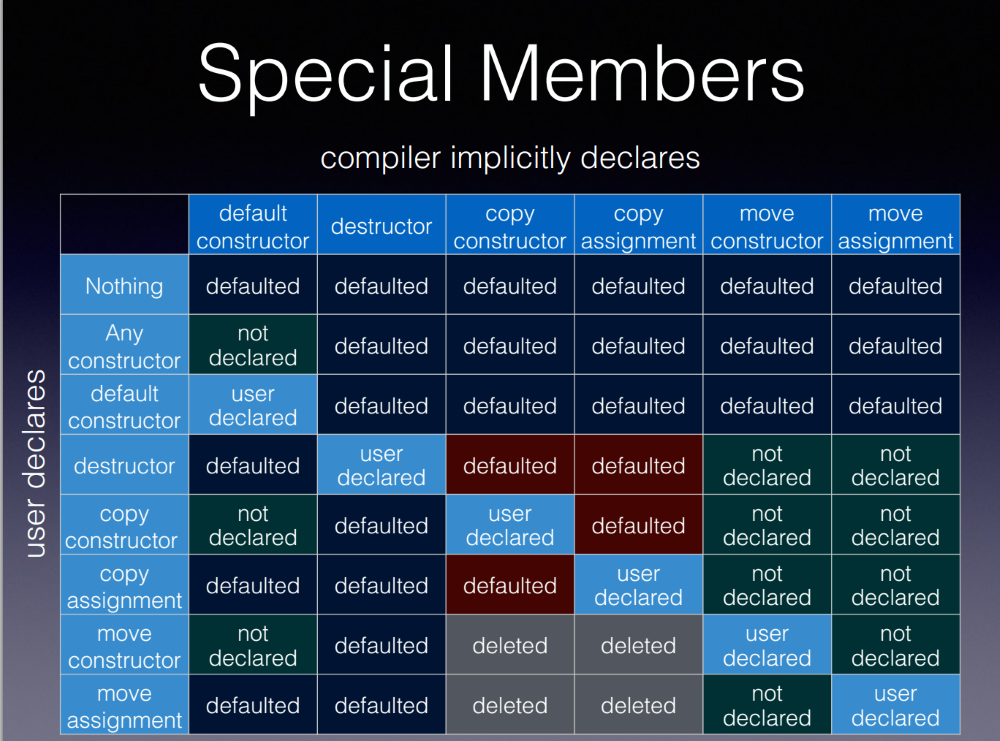
\includegraphics[width=40px]{https://prod-files-secure.s3.us-west-2.amazonaws.com/7761b648-9b3c-4888-9697-03086edc25f6/f8f82578-7099-4392-b79c-17fc9e1f78de/immagine.png}
\end{neonlisting}
\end{itemize}

\subsection{The \texttt{inline} Directive}

In C++, the \texttt{inline} keyword can be applied to free functions (functions that are not members of any class) to suggest that the function should be inlined by the compiler. This means that the compiler replaces function calls with the actual function code at the call site, potentially leading to better performance, especially for small, frequently used functions.

\begin{neonlisting}[language=C++]{Inline Function Example}
// Inline function declaration for a free function.
inline int add(int a, int b) {
    return a + b;
}

const int result = add(5, 7); // Calls the inline function.
std::cout << "Result: " << result << std::endl;
\end{neonlisting}

\begin{itemize}
    \item \textbf{Function size}: Inlining is most effective for small functions. For larger functions, inlining can lead to code bloat and may not improve performance.
    \item \textbf{Compiler's discretion}: The \texttt{inline} keyword is a \textbf{suggestion} to the compiler, and the compiler can choose whether or not to inline the function based on optimization settings and other factors.
    \item \textbf{Header files}: If you define \texttt{inline} functions in header files, be cautious about including the same header in multiple source files. It can lead to multiple definitions if not managed properly. Using header guards helps prevent this issue.
    \item \textbf{Balancing readability}: While inlining can improve performance, it should be used judiciously. Overusing inline for functions that don't provide significant performance benefits can lead to less readable code due to poor code organization.
\end{itemize}

\textbf{Pros of using} \texttt{inline}

\begin{itemize}
    \item \textbf{Potential performance improvement}: Inlining small functions can eliminate the function call overhead and improve runtime performance.
    \item \textbf{Avoiding multiple definitions}: When the same inline function is defined in multiple translation units (source files), the One Definition Rule (ODR) allows the multiple definitions to be treated as equivalent, which avoids linker errors.
\end{itemize}

In summary, you can use the \texttt{inline} keyword to suggest to the compiler that it should consider inlining the function for potential performance improvement. However, it's essential to balance performance considerations with code readability and maintainability.

\subsection{In-Class and Out-of-Class Definitions}

In C++, member functions of a class can be defined either in-class (inline) or out of class. Each approach has its use cases and implications.

\textbf{In-class (inline) Definition}

Member functions are defined within the class declaration itself, typically in the header file. This is common for short, simple functions that are typically one-liners or very concise.

\begin{neonlisting}[language=C++]{In-Class Definition Example}
// my\_class.hpp
class MyClass {
public:
    // inline keyword is implicit here.
    int add(int a, int b) {
        return a + b;
    }
};
\end{neonlisting}

The previous code is equivalent to the following:

\begin{neonlisting}[language=C++]{In-Class vs Out-of-Class Definition Example}
// my\_class.hpp

class MyClass {
public:
    int add(int a, int b);
};

// inline keyword is implicit here.
int MyClass::add(int a, int b) {
    return a + b;
}
\end{neonlisting}

\textbf{Pros}

\begin{itemize}
    \item Compact and concise code.
    \item Compiler may choose to inline the function for performance.
\end{itemize}

\textbf{Cons}

\begin{itemize}
    \item May lead to code bloat if used extensively with large functions.
    \item Changes to the function may necessitate recompilation of all translation units that include the header.
\end{itemize}

\textbf{Out-of-Class Definition}

Member functions are declared in the class declaration (in the header file) and defined separately in the source file (.cpp file). Typically used for functions with larger implementations or when you want to separate interface from implementation.

\begin{neonlisting}[language=C++]{Out-of-Class Definition Example}
// my\_class.hpp

class MyClass {
public:
    int add(int a, int b);
};
\end{neonlisting}

\begin{neonlisting}[language=C++]{Out-of-Class Definition Example Continued}
// my\_class.cpp

#include "my\_class.hpp"

int MyClass::add(int a, int b) {
    return a + b;
}
\end{neonlisting}

\textbf{Pros}

\begin{itemize}
    \item Separation of interface from implementation for cleaner code organization.
    \item Changes to the function implementation \textbf{do not} require recompilation of all translation units that include the header.
\end{itemize}

\textbf{Cons}

\begin{itemize}
    \item Slightly more verbose in terms of code.
    \item Requires separate source file for function definitions.
\end{itemize}

\textbf{Best Practices}

\begin{enumerate}
    \item Use in-class (\texttt{inline}) definitions for very short and simple functions (e.g., accessors, mutators) to potentially benefit from inlining.
    \item Use out-of-class definitions for larger or more complex functions to keep the header files clean and to separate interface from implementation.
    \item Consider code readability and maintainability when making a choice.
\end{enumerate}

In practice, a combination of both in-class and out-of-class definitions is often used, with the goal of keeping the code organized, maintainable, and efficient.

\subsection{Encapsulation and Access Control}

Data encapsulation is a fundamental concept in OOP that involves bundling data (attributes) and methods (functions) that operate on that data into a single unit called an object. Encapsulation helps hide the internal details of an object and exposes only the necessary functionality through well-defined interfaces.

\begin{neonlisting}[language=C++]{Encapsulation Example}
class BankAccount {
public:
    BankAccount(std::string account_holder, double balance) : account_holder(account_holder), balance(balance) {}

    void deposit(double amount) {
        balance += amount;
    }

    double get_balance() const {
        return balance;
    }

private:
    std::string account_holder;
    double balance;
};
\end{neonlisting}

\textbf{Access Specifiers}

C++ provides access specifiers to control the visibility and accessibility of class members (variables and methods). These access specifiers enforce encapsulation and access control within the class.

\begin{itemize}
    \item \texttt{public}: Members declared as public are accessible from any part of the program. They form the class's public interface.
    \item \texttt{private}: Members declared as private are not accessible from outside the class. They are used for internal implementation details.
    \item \texttt{protected}: Members declared as protected are accessible within the class and by derived classes (in \textbf{inheritance} scenarios).
\end{itemize}

\begin{neonlisting}[language=C++]{Access Specifiers Example}
class MyClass {
public:
    int public_var;    // Public member variable.
    void public_func() { // Public member function.
        // ...
    }

private:
    int private_var;    // Private member variable.
    void private_func() { // Private member function.
        // ...
    }
};
\end{neonlisting}

\subsection{Getter and Setter Methods}

Getter and setter methods, also known as accessors and mutators, are used to control access to private member variables.

\begin{itemize}
    \item \textbf{Getter} methods allow reading the values of private variables.
    \item \textbf{Setter} methods enable modifying those values in a controlled manner.
\end{itemize}

They are commonly used for encapsulation and access control.

\begin{neonlisting}[language=C++]{Getter and Setter Example}
class TemperatureSensor {
public:
    double get_temperature() const {
        return temperature;
    }

    void set_temperature(double new_temperature) {
        if (new_temperature >= -50.0 && new_temperature <= 150.0) {
            temperature = new_temperature;
        } else {
            std::cout << "Invalid temperature value!" << std::endl;
        }
    }

private:
    double temperature;
};
\end{neonlisting}

\subsection{Friend Classes}

A \texttt{friend} class is a class that is granted access to the private members of another class. This access allows the \texttt{friend} class to operate on the private members of the class it is friends with.

\begin{neonlisting}[language=C++]{Friend Classes Example}
class Circle {
public:
    friend class Cylinder; // Cylinder class is a friend of Circle.

    Circle(double r) : radius(r) {}

    double get_area() const {
        return 3.14159265359 * radius * radius;
    }

private:
    double radius;
};
\end{neonlisting}

\begin{neonlisting}[language=C++]{Friend Classes Example Continued}
class Cylinder {
public:
    Cylinder(const Circle &circle, double height) : circle(circle), height(height) {}
    
    double get_volume() const {
        // Accessing the private member 'radius' of the Circle class.
        return circle.radius * circle.radius * height;
    }

private:
    double height;
    const Circle circle;
};

Circle circle{1.0};
Cylinder cylinder{circle, 0.5};
const double volume = cylinder.get_volume();
\end{neonlisting}

\subsection{Operator Overloading}

Operator overloading is a feature in C++ that allows you to define custom behaviors for operators when used with objects of your own class. In essence, it enables you to extend the functionality of operators beyond their predefined meanings, making objects of your class work with operators in a way that makes sense for your class's context.

Operator overloading can improve code readability and maintainability by allowing you to write more natural and expressive code. It lets you use operators like \texttt{+}, \texttt{-}, \texttt{*}, \texttt{/}, and \textbf{many} others to perform operations specific to your class, just as you would with built-in data types.

\begin{neonlisting}[language=C++]{Operator Overloading Example}
class Complex {
public:
    // ...
    
    Complex operator+(const Complex& other) {
        Complex result;
        result.real = this->real + other.real;
        result.imag = this->imag + other.imag;
        return result;
    }

private:
    double real;
    double imag;
};

Complex a{2.0, 3.0};
Complex b{1.0, 2.0};
Complex c = a + b; // Using the overloaded '+' operator.
\end{neonlisting}

While you can overload \href{https://en.wikipedia.org/wiki/Operators_in_C_and_C%2B%2B}{many C++ operators}, here are some of the most commonly overloaded operators:

\begin{itemize}
    \item Arithmetic operators: \texttt{+}, \texttt{-}, \texttt{*}, \texttt{/}, \texttt{\%}, etc.
    \item Comparison operators: \texttt{==}, \texttt{!=}, \texttt{<}, \texttt{>}, \texttt{\textless=}, \texttt{\textgreater=}, \texttt{<=>} (since C++20), etc.
    \item Assignment operators: \texttt{=}, \texttt{+=}, \texttt{-=}, etc.
    \item Increment/decrement operators: \texttt{++}, \texttt{--}.
    \item Stream insertion/extraction operators: \texttt{<<}, \texttt{>>} (used for input and output).
    \item Function call operator: \texttt{()} (used to create objects that act like functions).
    \item Subscript operator: \texttt{[]} (used to access elements of an array-like class).
    \item Member access operator: \texttt{->} (used to access members of an object through a pointer).
\end{itemize}

You can overload operators as member functions or non-member functions.

\begin{itemize}
    \item When overloaded as a \textbf{member function}, the left operand is an object of the class, and the right operand is passed as a parameter.
    \item When overloaded as a \textbf{non-member function}, both operands are passed as parameters. This is often preferred when the left operand is not an object of the class you're overloading the operator for. Sometimes, you may need to access private members of a class when overloading an operator. In such cases, you can declare the overloaded operator function as a friend of the class. This allows the operator function to access the private members of the class.
\end{itemize}

\begin{neonlisting}[language=C++]{Operator Overloading as Non-Member Function Example}
class MyClass {
public:
    MyClass(int v) : value(v) {}

    // Declaring the '<<' operator as a friend function.
    friend std::ostream& operator<<(std::ostream& os, const MyClass& obj);

private:
    int value;
};

// Overloading the '<<' operator as a non-member function (outside the class).
std::ostream& operator<<(std::ostream& os, const MyClass& obj) {
    os << obj.value;
    return os;
}

MyClass obj;
std::cout << obj << std::endl;
\end{neonlisting}

\textbf{Operator Overloading: Best Practices}

\begin{enumerate}
    \item \textbf{Operators that cannot be overloaded}
    
    Some operators, like \texttt{::}, \texttt{.*}, and \texttt{? :}, cannot be overloaded.
    
    \item \textbf{Don't change the basic meaning of an operator}
    
    Overloading should make sense in the context of your class. For example, overloading \texttt{+} for string concatenation is intuitive, but overloading it for subtraction is not.
    
    \item \textbf{Be mindful of operator precedence and associativity}
    
    Overloaded operators should follow the same precedence and associativity rules as their built-in counterparts (such as in expressions like \texttt{2 * 3 + 1}).
    
    \item \textbf{Avoid excessive overloading}
    
    Overloading too many operators can make your code less readable and harder to maintain. Focus on overloading the operators that provide significant benefits.
\end{enumerate}

\begin{definitionblock}
    
    \texttt{class} vs. \texttt{struct}
    
    ---
    
    In C++, both \texttt{class} and \texttt{struct} are used to define classes. The only difference between them is the default access specifier:
    
    \begin{itemize}
        \item In a \texttt{class}, members are private by default.
        \item In a \texttt{struct}, members are public by default.
    \end{itemize}

\end{definitionblock}
    
\begin{neonlisting}[language=C++]{class vs struct Example}
class MyClass {
    int x; // Private by default.
public:
    int y; // Public.
};

struct MyStruct {
    int x; // Public by default.
private:
    int y; // Private.
};
\end{neonlisting}